\documentclass[11pt,letterpaper]{article}
\usepackage[T1]{fontenc}
\usepackage[utf8]{inputenc}
\usepackage{lmodern,microtype}
\usepackage[margin=0.88in,headheight=15pt]{geometry}
\usepackage{amsmath,amssymb,booktabs,longtable,array,tabularx}
\usepackage{graphicx,xcolor,xurl,enumitem,caption,fancyhdr,float}
\usepackage[colorlinks=true,linkcolor=AlphaPurple,urlcolor=AlphaPurple,citecolor=AlphaPurple]{hyperref}
\definecolor{AlphaPurple}{HTML}{7046C7}
\definecolor{AlphaNavy}{HTML}{162238}
\definecolor{AlphaMist}{HTML}{F3F0FA}
\definecolor{AlphaTeal}{HTML}{087F8C}
\hypersetup{pdftitle={AGI ALPHA Flywheel: The Second Investment},pdfauthor={Assistant-assisted research for the MontrealAI project},pdfsubject={A frozen production experiment and strategic-market test of operating-funded reinvestment},pdfkeywords={capability investment, operating surplus, causal comparison, negative result, reproducibility}}
\pagestyle{fancy}
\fancyhf{}
\fancyhead[L]{\small\color{AlphaPurple}\textbf{AGI ALPHA} $\boldsymbol{\infty}$}
\fancyhead[R]{\small\color{AlphaNavy}The Second Investment}
\fancyfoot[L]{\small Research record \textbullet\ 26 October 2026}
\fancyfoot[R]{\small\thepage}
\renewcommand{\headrulewidth}{0.3pt}
\setlength{\parindent}{0pt}
\setlength{\parskip}{5pt}
\setlength{\emergencystretch}{2em}
\setlist{nosep,leftmargin=*}
\captionsetup{font=small,labelfont=bf}
\newcolumntype{Y}{>{\raggedright\arraybackslash}X}
\newcommand{\USD}[1]{\$#1}
\DeclareRobustCommand{\artifact}[1]{\texttt{#1}}
\newcommand{\resultbox}[1]{\begin{center}\colorbox{AlphaMist}{\parbox{0.94\linewidth}{\vspace{5pt}#1\vspace{5pt}}}\end{center}}
\title{\vspace{-20pt}\color{AlphaPurple}\Large\textbf{AGI ALPHA FLYWHEEL}\par\vspace{8pt}\color{AlphaNavy}\Huge\textbf{The Second Investment}\par\vspace{10pt}\large An executed test of operating-funded capability growth}
\author{Assistant-assisted research prepared for the MontrealAI project\\\small Coordinated through AGI-Alpha-Agent-v0 issue \#4850}
\date{26 October 2026 \quad\textbullet\quad Frozen research edition v1}

\begin{document}
\maketitle
\thispagestyle{empty}
\begin{abstract}
\noindent Useful work can finance capability growth only when a distinct next asset is both affordable from collected operating resources and worth more than its complete cost. We test that mechanism by continuing an existing AGI ALPHA enterprise model and constructing an actual second capability: a source-bound, full-lock dependency metadata preflight, built by adopting ordinary pip and packaging tools and retained through the unchanged SUCCESSOR $\Omega$ Workbench. A bounded four-choice screen, independent acceptance contract, source freeze and six fresh research-proposed lock substitutions precede confirmation. The strong incumbent, retained capability and independent conventional builder each deliver six accepted answers: four metadata-consistent configurations and two declared-project constraint conflicts. The retained workflow produces no additional accepted outcome and is slower on every measured question; mean complete service time is 1.340 seconds versus 1.135 for the incumbent and 1.175 for the conventional builder. No human-effort saving is observed.

We bind these results to a separately frozen strategic-market continuation: 1,920 paired worlds, 5,760 enterprise histories, 13 conditions, 24 fresh seeds, three explicit complete-cost scenarios and an unidentified-cost boundary. All branches inherit the same first-asset enterprise. There are 114 operating-funded research attempts per treatment across the designed grid, but no financially qualifying second investment. In a preselected history, a \USD{25.97} attempt fits \USD{82.74} of generated funds, receives 15 modeled uses, incurs \USD{1.50} upkeep and loses \USD{27.47} relative to continuing the incumbent. The \USD{103.85} reference cost is unaffordable at that checkpoint. This is an executed negative reinvestment result, not a completed Flywheel. Actual customer receipts remain zero; actual all-in monetary cost remains unidentified. Source, failures, usable bilingual packets, cash histories and reproduction tools accompany the paper.
\end{abstract}

\resultbox{\textbf{Finding.} The asset works within its registered metadata scope. It does not establish a worthwhile second investment. Cash availability, technical usefulness, historical cost recovery and incremental repayment are different claims.}

\section{The economic mechanism and the customer outcome}

A maintainer deciding whether to change a dependency lock needs a defensible next action. The existing first capability supplies a scoped component-behavior decision with original consumer definitions, exact environments, observed tests and a proposed component-lock patch. Its useful result is evidence that a particular declared contract was preserved or violated, together with the remaining qualification work. It does not certify the whole application. The proposed second asset answers a distinct remaining question: are all distributions in a proposed native lock consistent with the declared project roots and active dependency metadata on the specified interpreter?

That question is useful before installation. A substantiated negative decision can prevent an inadmissible proposal; a positive metadata decision can support proceeding to broader qualification. Neither outcome proves application correctness. The experiment preserves that distinction in the acceptance contract, raw certificates, native records and user-facing English/French packets. It does not replace the broader maintainer outcome with a count of package names or assert that metadata consistency is release approval.

The financial claim requires more than an asset and a positive cash balance. Let $G_t$ be resources generated by operations and available at the decision time, $K$ the complete one-off second-asset cost, $M$ its lifetime upkeep, and $\Delta\Pi$ its paired, project-inclusive incremental profit. A bounded modeled reinvestment cycle requires
\begin{equation}
K\leq G_t,\qquad \Delta\Pi>0,
\end{equation}
together with executed useful production, independent acceptance, an identified constructed asset, a defensible workload and complete cost accounting. Funding is a cash constraint. Repayment is a causal value constraint. The same dollar cannot be counted both as an original seed contribution and as later earned revenue.

Three questions must therefore remain separate. Deploying an already built asset can be prospectively beneficial. That benefit need not recover the historical research bill. Even when operations accumulate resources, the next proposed asset can fail to earn its own cost. This study tests the third question while preserving the earlier answers. A gain over the strong incumbent would establish investment value; only an additional gain over the conventional builder would support a distinctive improvement-method advantage. Conventional parity is not itself a reason to reject a useful investment.

\section{Starting evidence and continuity}

The study begins from the coordinated records of AGI-Alpha-Agent-v0, AGI-Fleet-Linux, AGIJobsv0 and AGIJobManager, using pinned source identities rather than a moving release claim \cite{coordination,prior}. The current study and lock checkout is Alpha commit \texttt{b1d52a7}; the unchanged native Workbench and original consumer snapshot are inherited from \texttt{eb07086ac42799ff45f7b1c946a2f7c514bd3bbc}. The retained first producer is identified by SHA-256 \texttt{0b4eb1ae2392\ldots}. Its source and prior acceptance records are preserved in the companion. Fleet, Jobs and Manager supply existing bounded planning, evidence and admission conventions; they are not evidence of connected commercial activity. No active application, operator, Journal or settlement runtime was started or restarted for this study.

\begin{table}[htbp]
\centering\small
\begin{tabularx}{\linewidth}{@{}p{0.23\linewidth}p{0.16\linewidth}Y@{}}
\toprule
Preserved study & Paired worlds & Evidence retained \\
\midrule
Primary strategic market & 2,088 & Negative adoption/profit result under the registered primary design. \\
Exploratory expansion & 2,472 & Six seed-funded first-asset adoptions; no positive condition mean. Exploratory, not confirmation. \\
Policy diagnostic & 1,920 & Conditional prospective deployment benefit; reused seeds and changed policy interpretation remain explicit. \\
Fresh deployment continuation & 3,072 & Conditional first-asset benefit and historical loss; no second asset or second investment. \\
Prior second-asset screen & Three choices & No justified second productive capability. Its 321.81-second review window is not measured human labor. \\
\bottomrule
\end{tabularx}
\caption{Earlier evidence is preserved, not pooled with the new confirmation or relabeled as second-investment success. Exact original summaries and their hashes are included under \artifact{heritage/prior-market-results/}.}
\end{table}

The preceding fresh conditional reference reported mean prospective profit of \USD{151.70}, a \USD{173.67} paired first-deployment advantage, three losses among 24 seeds and mean full-history profit of approximately $-\USD{209.82}$. Its generated-funds figures were ceilings before unknown further discovery cost. The new study does not remove that cost uncertainty, transfer the earlier first-asset saving to a second asset or use a later terminal cash balance to fund an earlier decision.

The first capability was actually produced in a supplied research environment; complete research billing and active human attention were not observed. In the inherited economic model, original seed capital is \USD{1,000}, the reserve is \USD{200}, opening historical research is priced at \USD{361.52}, and adoption of the existing first asset costs \USD{32.69}. The historical allowance is four assumed hours at \USD{65.38} plus \USD{100} authoring; it is not a measured invoice or a finite empirical bound. The first asset enables useful component evidence and removes a repeated explicit researcher-finalization step in the previous experiment. Its conventional counterpart achieved the same six accepted outcomes. Earlier response intervals were not active labor and are not retrospectively priced as such.

\section{A finite search, with ordinary software as a serious alternative}

Before discovery, the research envelope limited work to four choices, 30 minutes of screening, one selected capability, one fresh confirmation cohort, at most four concurrent assistant roles and a three-hour deadline ending at 20:57 UTC. No paid commitment, new credential, outreach, financial action or security change was authorized. A negative finding ends this envelope; an unfavorable result does not authorize replacing the offering, changing prices or extending the horizon.

The observed burden is precise. Prior component packets leave full native-lock qualification unsupported. The current native lock has 41 distributions; the earlier component contract's 61 behavioral assertions are a different count. The repository already has hash-locked installation and pip checking. A development preflight using a legitimate shared wheel cache completed in 0.7604 seconds of wall time. Therefore a new asset cannot be justified merely by automating a supposedly expensive resolver step.

\begin{table}[htbp]
\centering\small
\begin{tabularx}{\linewidth}{@{}>{\raggedright\arraybackslash}p{0.22\linewidth}YY@{}}
\toprule
Choice & Useful outcome and strongest alternative & Decision within the envelope \\
\midrule
Maintain incumbent & Continue scoped component decisions; use ordinary pip and existing installer diagnostics. & Mandatory no-investment comparison. No new retained construction is assumed. \\
Adopt pip preflight & Exact whole-lock metadata evidence and project-root witnesses; compare with direct pip and a conventional wrapper. & One bounded prototype selected for falsification, not financially admitted in advance. \\
Custom metadata resolver & Same consistency question; ordinary pip and packaging already implement relevant semantics. & Rejected before construction: no observed advantage justifies duplicate semantics and upkeep. \\
Full application qualification & Broader auth, persistence, mission and platform assurance; existing release/CI lane is the strong alternative. & Potentially useful, but closure, burden and cost are unmeasured and active owners must not be duplicated. \\
\bottomrule
\end{tabularx}
\caption{The screen includes adoption and no investment. Discovery, rejected choices, failed attempts and common research work remain cost categories. Unknown future construction and reuse are not zero-filled.}
\end{table}

The TRANSFORMATIONAL INTELLIGENCE question was whether a different information source and representation could remove the need to launch the whole application for this narrow question. Declarative wheel metadata, ordinary resolver evidence and unchanged project constraints can do so. That is a useful change of production method, but the incumbent can adopt the same representation. A broader application claim cannot be substituted for the narrower result. The method transformation succeeds technically without creating a demonstrated economic advantage.

Future lock changes are plausible, supported by an actual repository maintenance obligation and external descriptions of recurring dependency work. Neither scheduled checks nor six research substitutions establish paid recurrence. For the selected asset, the prospective repayment mechanism was an incremental accepted outcome or measured recurring resource reduction. Its explicit falsifier was strong A delivering the same scope at no higher recurring cost. That falsifier occurred.

\section{Construction and frozen production confirmation}

\subsection{What was actually built}

The B implementation verifies declared input and wheel hashes, creates a job-specific view of the existing wheel cache, preserves requested extras and exact roots, invokes ordinary pip in dry-run/report mode, and records the evidence. A separately authored verifier reads exact wheel \texttt{METADATA} and tags, checks project roots, Python requirements, markers, recursive extras and active dependency edges, and compares the report with the selected inventory. Missing, stale, unsupported or contradictory evidence cannot masquerade as a complete positive decision.

The retained adapter is registered in the copied, unchanged local SUCCESSOR $\Omega$ Workbench. Its output includes a source-bound mission pack and artifact references. It does not obtain new authority. All six B packs remain \texttt{HOLD}, with empty authority and active proof, disconnected settlement and historical-import inspection status. These native states are evidence boundaries, not an administrative reason for the economic rejection. The asset fails its investment case because incremental value was not demonstrated.

The source was authored by assistant researchers using local tools. The system's native engine compiles and executes the registered work; it did not autonomously invent pip, its verifier or the experimental design. The conventional builder was a separate assistant role, with the same ordinary tools, shared cache and bounded resource access, and without seeing B's implementation before construction. It is not a hired-human benchmark. Native execution made zero runtime model calls; assistant authoring inference occurred outside that execution and its bill remains unknown.

\subsection{Comparisons and acceptance}

New A keeps the strong existing workflow and uses direct ordinary pip, explicit project-constraint checks and a study-only recorder. B uses the retained native adapter. C uses the independently built conventional wrapper. All receive the same frozen acceptance checker and valid cache. The recorder and shared checker were research contributions, not proof that a newly constructed commercial A system is free. Their construction and scrutiny are included in the complete-category uncertainty and scenario allocations. Per-job verification resources are measured in every arm.

The creator--critic--verifier process followed the supplied DOCX's requirement for source-backed, consequential objections. It found a native headline that could disagree with verified acceptance, an absolute-path input refusal in C, and gaps in driver source/job binding and partial-output preservation. Corrections occurred before fresh target metadata was acquired. Superseded unexecuted development freezes, failed attempts and review records remain in the archive. The verifier's 24 synthetic controls cover false consistency, missing data, markers, extras, Python constraints, malformed evidence and transitive problems; they are not fresh customer jobs.

The frozen acceptance standard was a complete source-grounded metadata decision, including a valid negative decision. The verifier was independently authored by a separate assistant role before fresh inspection, but it is the same shared validator in all arms. Later archive recomputation is a custody check using that validator, not a second independent oracle, external peer review or customer acceptance.

\subsection{Fresh inputs and execution}

For each of six previously untested families, the protocol selected the immediately previous stable, non-yanked release below the current pin. Selection inspected identity, availability and wheel compatibility before predecessor dependency metadata or outcomes. Other 40 versions and the project roots remained fixed. These are prospectively selected, research-proposed historical substitutions. They are not actual historical application lockfiles, real maintainer requests or observed market orders.

\begin{table}[htbp]
\centering\small
\begin{tabular}{@{}llll@{}}
\toprule
Changed family & Current pin & Proposed pin & A/B/C accepted decision \\
\midrule
cryptography & 50.0.1 & 50.0.0 & Project-root conflict \\
eth-account & 0.13.7 & 0.13.6 & Project-root conflict \\
prometheus-client & 0.26.0 & 0.25.0 & Metadata consistent \\
pydantic-settings & 2.15.0 & 2.14.2 & Metadata consistent \\
PyYAML & 6.0.3 & 6.0.2 & Metadata consistent \\
uvicorn & 0.53.0 & 0.52.4 & Metadata consistent \\
\bottomrule
\end{tabular}
\caption{Six questions, eighteen arm evaluations and zero new customer orders. Missing releases, missing wheels or failures would remain in the cohort; no outcome-dependent replacement was allowed.}
\end{table}

The exact target was CPython 3.12.14 on the recorded Linux x86-64 environment, with the project's \texttt{chain} extra. The execution tool versions were pip 26.2.2 and packaging 26.3. The three run orders were ABC, BCA and CAB, each used twice. Each arm ran once per question. Complete service timing includes independent verification and B's native orchestration; inclusive CPU receipts avoid adding nested command time twice. No human or customer time was inferred from elapsed machine time. Source hashes were checked before and after confirmation, and registered job/result/certificate bindings were checked after execution.

\section{Executed useful outcomes and the absent incremental benefit}

All 18 outputs passed the registered scope. The two conflicts are exact, useful root-version rejections: \texttt{cryptography==50.0.0} violates \texttt{cryptography>=50.0.1,<51}, and \texttt{eth-account==0.13.6} violates \texttt{eth-account>=0.13.7,<0.14}. These minimum requirements were already visible during development. The findings are not newly discovered upstream bugs or runtime regressions. All eighteen pip commands exited zero; the separate project-root checks supply the negative evidence.

The other four proposals were consistent with the registered metadata checks. They still require application qualification. A source-bound JSON certificate, raw resolver output, exact input lock and readable bilingual packet make each result usable and inspectable. The common post-evaluation presentation renderer is a research/publication contribution. Its work is not credited as a B-specific benefit or added to the primary acceptance count.

\begin{table}[htbp]
\centering
\begin{tabular}{@{}lrrr@{}}
\toprule
Measure & A: incumbent & B: retained & C: conventional \\
\midrule
Accepted scoped outcomes & 6/6 & 6/6 & 6/6 \\
Substantiated conflicts & 2 & 2 & 2 \\
Mean complete service, seconds & 1.135234 & 1.339685 & 1.175498 \\
Median complete service, seconds & 1.159387 & 1.371335 & 1.160239 \\
Mean inclusive CPU, seconds & 1.076644 & 1.320279 & 1.115226 \\
Measured human/customer saving & Unknown & Unknown & Unknown \\
\bottomrule
\end{tabular}
\caption{Descriptive same-host observations, including verification. Six accepted cases do not establish a field reliability rate. Earlier completion is distinct from additional eventual output; neither advantage is demonstrated for B.}
\end{table}

\begin{figure}[H]
\centering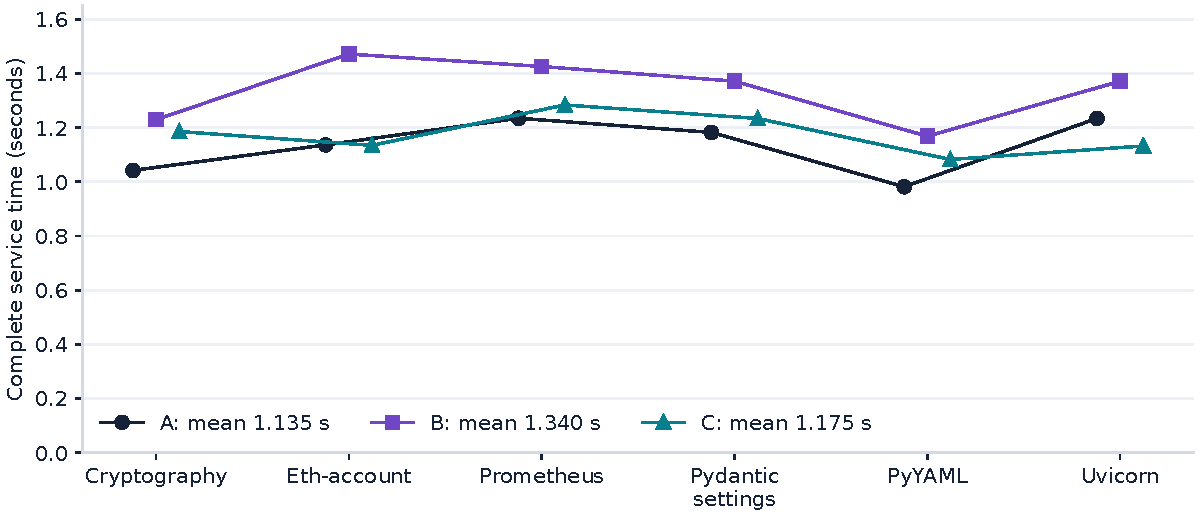
\includegraphics[width=\linewidth]{figures/production.pdf}
\caption{B was slower than A and C in all six recorded questions. Mean paired B--A difference is +0.204452 seconds; B--C is +0.164188 seconds. There is no population timing claim from one run per arm.}
\end{figure}

The production-derived economic effect is deliberately narrow. No provider-minute saving, customer-review saving, demand increase, quality increase or price premium is assigned. Crediting zero savings does not assert that actual human effort is zero. At an explicit diagnostic tariff of \USD{1} per CPU-hour, the mean B slowdown of 0.243635 CPU-seconds corresponds to a cost penalty of about \USD{0.00006768} per use. C's smaller mean slowdown corresponds to \USD{0.00001072}. Both round to zero in the integer-cent ledger; signed microcent residuals are retained. The largest B residual across executed modeled histories is \USD{0.00230112}. Ignoring that small penalty cannot manufacture a positive direct benefit.

The appended metadata stage does not replace the original service's timing. The inherited service measurement is 16.7994 wall seconds and 2.5392 CPU-seconds. Even appending the worst observed B stage leaves machine capacity far above the model's four enterprise slots per week. No additional sales or faster customer service is created from a nonbinding machine constraint.

\section{One finite ledger and complete-cost accounting}

Let $S$ denote original capital, $C_t$ cash, $R_t$ collected receipts, $E_t$ all accrued expenses, $O_t$ unpaid obligations, $r$ one reserve, and $H_0$ the historical opening research bill explicitly paid from seed before customer collections. The continuation uses
\begin{align}
C_t &= S+R_t-\text{paid expenses}_t,\\
G_t &= \max\{0,\min(C_t-O_t-r,\ R_t-E_t+H_0)\}.
\end{align}
The $H_0$ addback only identifies subsequent operating-generated funds. It does not reverse the historical cash payment, remove it from full-history profit, add new capital or forgive later search and construction costs. The reserve is applied once through the cash bound. Invoices and receivables are not collected funds. Refunds, corrections, defaults, upkeep and unpaid bills remain explicit.

Every new A/B/C branch begins from the existing first-asset B enterprise and its original history. New A never reverts to the earlier no-first-asset workflow. The implementation verifies exact shared histories before the second decision and exact correspondence between new A and the frozen original B. The original market engine remains byte-identical; nine disclosed insertions add continuation hooks. Independent controls cover cash reconciliation, reserves, refunds, delayed bills, signed regressions, unknown costs and complete research costs counted once.

\begin{table}[htbp]
\centering\small
\begin{tabular}{@{}lrrr@{}}
\toprule
One-off cost category, modeled USD & Low & Reference & High \\
\midrule
Prior unsuccessful discovery & 2.50 & 10.00 & 40.00 \\
New discovery & 2.50 & 10.00 & 40.00 \\
Rejected candidates/failed attempts & 1.25 & 5.00 & 20.00 \\
Construction & 6.54 & 26.15 & 104.60 \\
Independent verification/corrections & 3.27 & 13.08 & 52.32 \\
Second-asset integration & 1.64 & 6.54 & 26.16 \\
Other researcher contributions & 3.27 & 13.08 & 52.32 \\
Authoring model and tools & 5.00 & 20.00 & 80.00 \\
\midrule
Total one-off & 25.97 & 103.85 & 415.40 \\
Upkeep per active week & 0.06 & 0.25 & 1.00 \\
\bottomrule
\end{tabular}
\caption{Complete-category scenario allocations, identical for B/C; not observed invoices or empirical bounds. The actual-cost profile keeps every category unknown. Failure and common research costs cannot disappear because deployment is declined.}
\end{table}

The reference construction, verification, integration and other researcher amounts correspond approximately to 24, 12, 6 and 12 assumed minutes at \USD{65.38}/hour. These durations are scenario choices, not measurements of active attention. The low allocation is one quarter of each reference amount rounded to cents; the high allocation is four times reference. New model/API purchases are zero, but that does not make supplied assistant inference or research labor free. Unknown actual costs remain null and prevent an affirmative actual-cost financing claim.

Two policies expose different decisions. Under \emph{adaptive} search, affordable discovery costs are paid once during weeks 26--40. Construction requires a positive forecast of complete-cost repayment and available generated funds. Past search is included in the repayment hurdle without being charged again. Under \emph{completed-research replay}, the model tests whether all costs of the already constructed research prototype fit generated funds at week 26. If affordable, it may record an \emph{operating-funded, unqualified research attempt}, even when the value gate fails. It never calls that an admitted investment. If unaffordable, it does not borrow later collections or insert a subsidy.

In either policy, any completed prototype cost not paid by the modeled enterprise remains an explicit outside-enterprise research contribution. It adds no enterprise cash and is deducted once from project-inclusive profit. Thus choosing not to deploy does not erase the actual research attempt. The no-investment enterprise is retained as the counterfactual, while study costs and project costs remain visible.

\section{Strategic market, calibration and frozen robustness design}

The existing model represents repeated procurement among the enterprise, competent human providers, competing AI, do-it-yourself/conventional tools and deferral. A buyer's offer utility is
\begin{equation}
U_{ij}=q_{ij}V_i-p_j-e_{ij}-d_{ij}-s_{ij}-(1-q_{ij})L_i,
\end{equation}
where $q$ is believed quality, $V$ useful outcome value, $p$ price, $e$ review effort, $d$ delay, $s$ switching/integration friction and $L$ error loss. Dominated offers are removed, nonpositive utility can be rejected, and a logit choice rule retains the option to defer. Procurement budgets, delayed quality feedback and temporary churn allow buyers to switch or stop purchasing. Competitors have costs, cash, capacity and response rules, including cheaper automation and undercutting. This is a behavioral strategic simulation, not a demonstrated Nash equilibrium, optimal strategy or estimated market share.

Calibration is evidence-grounded but incomplete. Official wage data anchor a labor-rate sensitivity; \USD{135,980} divided by an assumed 2,080 work hours gives approximately \USD{65.38}/hour, not a contractor bill rate \cite{bls}. Official pip and packaging documentation support the adopted method \cite{pip,metadata,pipcheck}. Dependabot and Renovate establish competent conventional alternatives \cite{dependabot,renovate}; GOV.UK documents an actual recurring maintenance obligation and an existing automated/review workflow \cite{govuk}. The preserved calibration manifest distinguishes such sources from unidentified willingness to pay, arrival intensity, customer attention, exact integration cost, task-level reliability and authoring expense. External sources support mechanisms and ranges, not measured AGI ALPHA demand.

The reference intentionally retains the earlier favorable conditional region: 12 modeled buyers, arrival probability 0.5, fixed \USD{20} price, logit choice, zero assumed initial buyer integration, \USD{1,000} original capital, \USD{200} reserve and 52 service weeks. Zero integration is an inherited assumption, not a measured absence of onboarding. Reference quality remains the earlier scenario probability 0.95, not 1.0 inferred from six accepted technical cases. Provider and buyer effort remain inherited assumptions, unchanged across treatment arms.

Thirteen predeclared conditions include the reference; arrival probabilities 0.25, 0.1 and zero; buyer integration of \USD{2.50} and \USD{5}; 13-week collections; a cheaper capable AI; a \USD{16} enterprise price; undercutting competitors; 20\% second-integration failure; \USD{2}/week second upkeep; and a quality shock beginning at week 26. Conditions are not selected after seeing their results. Three cost profiles and two policies yield 78 priced groups. Two additional reference groups retain actual costs as unknown. The 24 fresh seeds 8001--8024 produce exactly 1,920 paired worlds and 5,760 reported enterprise histories.

The source, protocol, cost profiles, production-derived effects and runner were publicly registered before market execution. Seed 8001 and all eight reference cost/policy combinations were selected in advance for explanation. The campaign completed in 39.11 seconds wall time and 43.00 seconds CPU, within a declared 180-second execution budget. There were no substituted seeds, dropped conditions, reruns or horizon extensions. After week 51, the finite model drains existing collections, refunds and obligations; it creates no new service work during settlement.

\section{Results: affordability does not establish repayment}

Across all 1,920 paired worlds, B and C each have zero qualifying second investments, zero adaptive construction admissions and zero direct second-asset repayment. There are 114 operating-funded completed-research attempts per arm across the designed grid, including three integration failures. Counts across deliberately varied conditions are not probabilities that a real firm could fund an investment.

\begin{table}[htbp]
\centering\small
\begin{tabular}{@{}lrrrrrr@{}}
\toprule
Cost profile & One-off & Funded & Mean $\Delta\Pi$ & 5th pct. & 95th pct. & Qualified \\
\midrule
Low & 25.97 & 11/24 & -30.17 & -59.97 & -12.31 & 0/24 \\
Reference & 103.85 & 3/24 & -107.56 & -139.03 & -103.85 & 0/24 \\
High & 415.40 & 0/24 & -415.40 & -415.40 & -415.40 & 0/24 \\
\bottomrule
\end{tabular}
\caption{Predeclared reference market, completed-research replay, 24 seeds per row. Dollar columns are modeled USD; $\Delta\Pi$ is B minus A project-inclusive profit. Actual unknown-cost results remain unidentified rather than zero.}
\end{table}

For the reference-cost replay, mean incremental project profit is $-\USD{107.56}$, median $-\USD{103.85}$, with 5th and 95th percentiles $-\USD{139.03}$ and $-\USD{103.85}$. The conditional Monte Carlo 95\% interval for that mean is approximately $[-\USD{113.45},-\USD{101.67}]$. This is simulation uncertainty conditional on assumptions, not a confidence interval for commercial profitability. The low-cost reference replay is affordable in 11/24 histories; reference cost in 3/24; high cost in none. All 24 paired project deltas in each reference cost cell are negative.

The adaptive policy admits no construction, as zero evidenced recurring savings cannot repay positive complete cost and upkeep. Search may still be paid where affordable. Once the already completed research is included, each priced adaptive project loses its one-off cost relative to A. No completed prototype is made free by a deployment decision. In 48 actual-unknown worlds, project-inclusive profit and its difference remain null.

\begin{figure}[!htbp]
\centering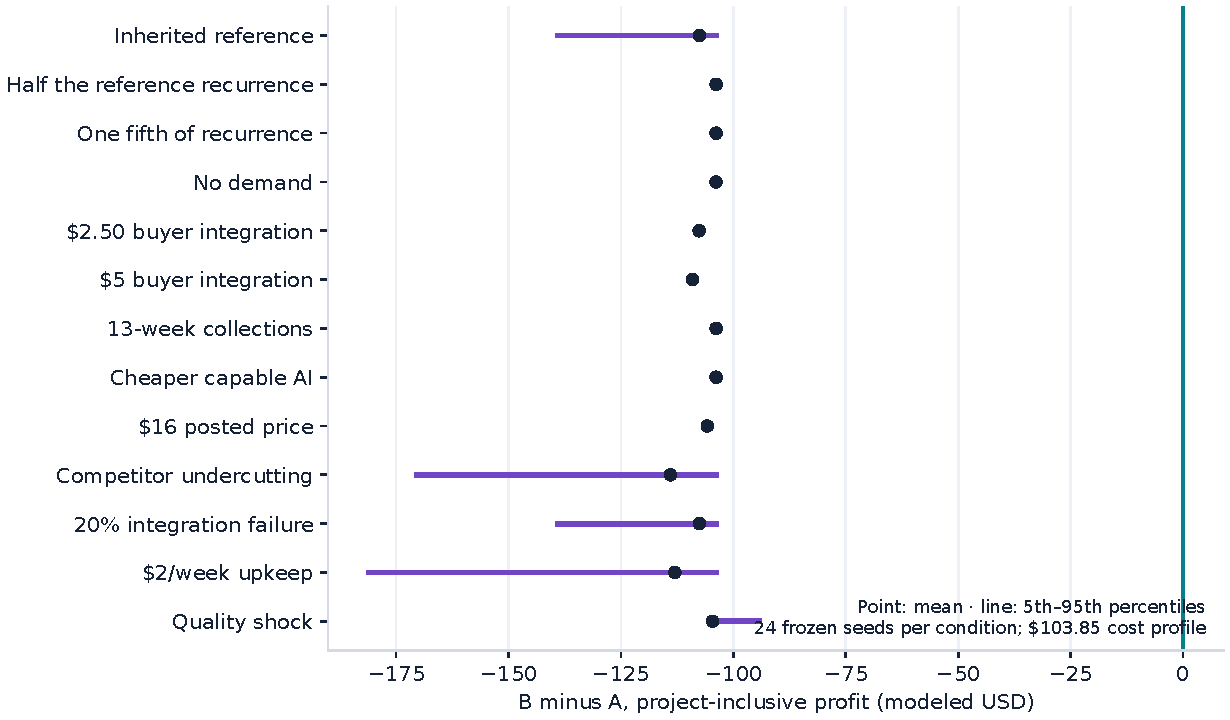
\includegraphics[width=\linewidth]{figures/robustness.pdf}
\caption{All 13 registered conditions at reference cost under completed-research replay. The empirical 5th--95th ranges describe 24 simulated histories per condition; they are not independent empirical market evidence or simultaneous confidence bands.}
\end{figure}

Among the 1,872 priced worlds, 1,870 B--A project deltas are negative and two are positive: +\USD{13.24} in the \USD{16}-price/low-cost replay at seed 8009 and +\USD{7.67} in the quality-shock/low-cost replay at seed 8017. Both remain unqualified, with zero direct second-capability saving and identical B/C cent-ledger results. Saved job, choice and feedback traces show how construction pauses perturb subsequent market histories; no separate pause-only ablation was registered or run. A favorable realized path is not evidence that the asset improved production. The exceptional histories are retained and explained rather than discarded. B/C project-inclusive cent-ledger parity holds in all 1,872 priced worlds; the separately recorded CPU residual favors C by a tiny amount, not a distinctive AGI ALPHA advantage.

\subsection{A preselected cash history}

At the week-26 decision in seed 8001, cumulative collections are \USD{340}, total accrued expenses are \USD{618.78}, and \USD{361.52} of those expenses are the already paid opening historical bill. Cash is \USD{721.22}, unpaid obligations zero and the reserve \USD{200}. Therefore
\begin{equation}
G_{26}=\min(721.22-200,\ 340-618.78+361.52)=\USD{82.74}.
\end{equation}
The reference \USD{103.85} complete prototype cannot be funded at that checkpoint. In its replay, the enterprise does not pay it, use it or borrow future funds. Its \USD{103.85} outside research contribution remains in project-inclusive results. The later terminal balance does not change the week-26 decision.

The low \USD{25.97} allocation can be funded. Paying its discovery and construction categories once leaves \USD{56.77} of generated funds. The asset activates in week 27, is used 15 times, and accrues \USD{1.50} upkeep over the remaining 25 active weeks. Both A and B finish with 34 accepted modeled outcomes and \USD{680} collections. B earns zero direct incremental benefit and loses \USD{27.47} versus A. Final cash is \USD{934.80} for B and \USD{962.27} for A; full-history profit is $-\USD{65.20}$ and $-\USD{37.73}$ respectively. Outstanding obligations are zero. A successful collection history can coexist with a bad reinvestment.

\begin{figure}[H]
\centering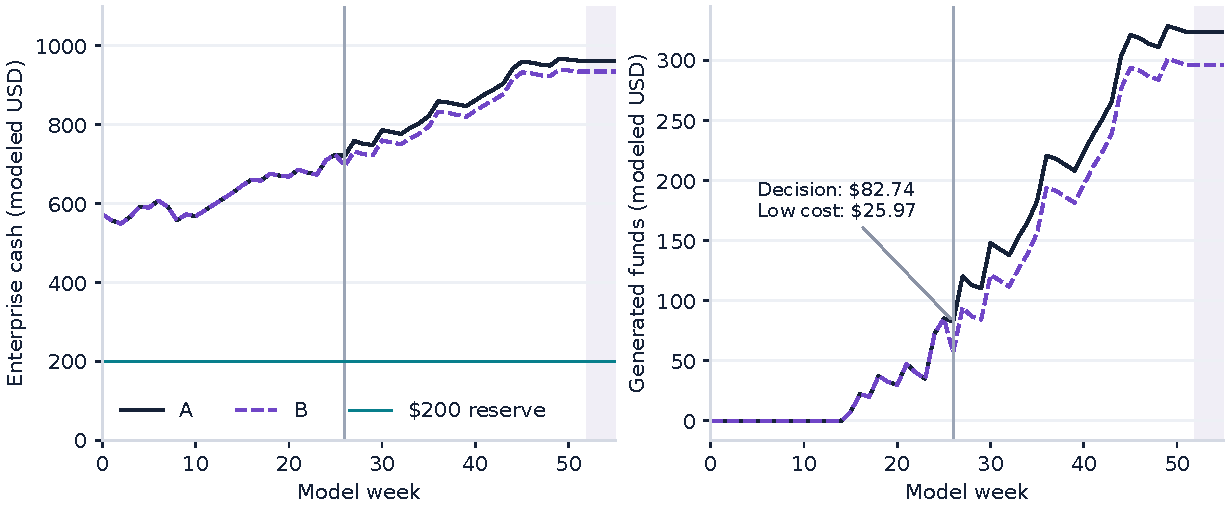
\includegraphics[width=\linewidth]{figures/finite-ledger.pdf}
\caption{The preselected seed-8001 low-cost research replay. Original seed, historical expenses, one reserve and subsequent operations share one ledger. The shaded final interval settles prior work only. All dollars are simulated.}
\end{figure}

In the new reference seeds, the incumbent first-asset enterprise's mean full-history profit is $-\USD{149.73}$. Adding back only the modeled historical opening cost for a prospective deployment view gives \USD{211.79}; this does not recover that historical expenditure or create a second-asset benefit. These fresh seeds do not replace the earlier study's numbers.

\section{Break-even conditions and the smallest missing evidence}

With $N$ defensible future uses, recurring incremental seller benefit $s$, upkeep $M$ and foregone contribution $F$, a necessary simple repayment condition is
\begin{equation}
Ns\geq K+M+F.
\end{equation}
It is not sufficient when price pressure, buyer switching, defaults and feedback change revenues. The paired ledger remains the primary financial comparison. Here supported $s$ is zero at cent precision, with a small negative CPU residual. No finite increase in recurrence repays positive $K$ from that effect alone. Lower costs cannot turn an absent benefit into a demonstrated positive one; zero demand cannot finance construction.

Using the preselected 15-use workload only as conditional arithmetic, low cost plus upkeep requires \USD{1.8313} incremental benefit per use before any downtime effect. At the assumed provider rate, that is approximately 1.681 minutes of verified active effort saved per use. The reference cost plus 25 weeks' upkeep is \USD{110.10}, requiring \USD{7.34}/use, or about 6.736 provider minutes. That reference asset was \emph{not} actually financed or used in the selected replay; this is a necessary-condition calculation on the preselected workload, not a completed result.

The unchanged market assumes only two residual provider minutes per delivered job after the first asset. Even eliminating both minutes would save about \USD{2.18}/use before tools; this is an assumed model ceiling, not a measured remaining burden. The reference-cost threshold therefore cannot be met by that labor channel alone on 15 uses. The low-cost threshold is mathematically possible but has no observed supporting time reduction. A future positive result would need a separately registered measurement showing that such a recurring burden exists and that the actual retained improvement removes it while preserving the same acceptance standard and complete costs. A measured customer benefit could also matter, but it would require supported seller capture rather than silently converting customer savings into revenue.

The smallest useful next observation is an actual pending maintainer decision with matched ordinary-tool and retained workflows, measured active attention, independent decision acceptance and complete applicable resource billing. A paid pilot is not logically necessary for a bounded modeled claim. A credible burden measurement and a full cost identification would let a new protocol test repayment within supported demand ranges. Reopening a broad application qualification branch would require its own baseline, owner coordination and finite acceptance closure. Neither step is performed here after the negative confirmation.

\section{Scope, preserved failures and reproducibility}

The negative result applies to this asset, task contract, ordinary-tool baseline and finite market model. It does not establish that no future capability can repay. Six technical questions are too few to estimate field reliability, and the two fresh negative cases exercise declared root constraints rather than transitive resolver failures. The synthetic controls provide separate engineering evidence. Prior component and joint-tuple outcomes are not counted again as fresh work. All complete monetary actual costs remain unidentified; the three priced scenarios expose their consequence without turning allowances into evidence.

The companion contains the actual B and C source, unchanged native closure, input identities and exact wheel bytes, raw production results, independent acceptance records, development corrections, cost profiles, all complete paired ledgers, protocols, figures, LaTeX and bilingual reports. A reader can inspect a decision, verify its source/certificate bindings, replay the frozen production cohort offline on the documented matching runtime, and rerun the registered economic code into a new output directory. Replays add zero new missions or customers. Dependency binaries are supplied in the full companion; the repository source/evidence edition is explicitly distinct from that offline bundle.

The paper and demonstration lead with the economic outcome. Their controls show predeclared scenario results and a separately labeled exploratory break-even calculator. Changing a hypothetical saving in the calculator does not overwrite the measured effect, admit an investment or produce customer receipts. An asset, invoice, modeled collection, reserve, finance gate and repayment result remain independently inspectable.

\resultbox{\textbf{Supported claim.} A distinct retained capability was constructed, executed on fresh registered inputs and checked. An additive, source-bound continuation shows that operating-generated modeled resources can finance some complete-cost research attempts, while this asset's demonstrated benefits do not repay those costs. The experiment does not establish a bounded reinvestment cycle, actual commercial receipts, autonomous invention, unlimited growth or self-acceleration. The justified action within this envelope is to retain the strong incumbent and preserve the failed investment evidence.}

\appendix
\section{Registered scenario results and exact accounting choices}

\begin{longtable}{@{}p{0.43\linewidth}rrrr@{}}
\caption{Reference-cost completed-research replay, modeled USD, 24 seeds per condition. No group has a qualifying investment.}\\
\toprule
Condition & Funded & Mean $\Delta\Pi$ & 5th pct. & 95th pct. \\
\midrule\endfirsthead
\toprule Condition & Funded & Mean $\Delta\Pi$ & 5th pct. & 95th pct. \\
\midrule\endhead
Inherited reference & 3/24 & -107.56 & -139.03 & -103.85 \\
Half the reference recurrence & 0/24 & -103.85 & -103.85 & -103.85 \\
One fifth of recurrence & 0/24 & -103.85 & -103.85 & -103.85 \\
No demand & 0/24 & -103.85 & -103.85 & -103.85 \\
\$2.50 buyer integration & 1/24 & -107.62 & -103.85 & -103.85 \\
\$5 buyer integration & 1/24 & -109.08 & -103.85 & -103.85 \\
13-week collections & 0/24 & -103.85 & -103.85 & -103.85 \\
Cheaper capable AI & 0/24 & -103.85 & -103.85 & -103.85 \\
\$16 posted price & 1/24 & -105.81 & -103.85 & -103.85 \\
Competitor undercutting & 9/24 & -113.99 & -170.41 & -103.85 \\
20\% integration failure & 3/24 & -107.56 & -139.03 & -103.85 \\
\$2/week upkeep & 3/24 & -113.03 & -181.08 & -103.85 \\
Quality shock & 3/24 & -104.63 & -103.85 & -94.23 \\
\bottomrule
\end{longtable}

The stronger AI condition uses initial price \USD{5}, cost \USD{1}, quality 0.97 and eight assumed review minutes. The undercutting condition uses the preserved competitor response tuple, including a 0.75 cost reduction and \USD{10} imitation cost. These are scenario mechanisms applied to all treatment arms, not newly observed competitor offers. The original human provider uses an assumed \USD{30}/hour and finite capacity; the DIY option includes review/effort rather than treating a free software license as costless work.

First adoption remains available under the inherited seed-funded policy and can be declined where its original forecast fails. Thus ``same first-asset enterprise'' means the same source, availability, financing policy and pre-second history, not an assumption that every zero-demand firm already activated it. The second asset's useful life is bounded to 26 weeks and the service horizon never exceeds 52 weeks. At a week-26 start with a one-week pause, at most 25 productive weeks remain.

The dedicated second-investment record must be used for second-asset repayment. Upstream direct-repayment counters aggregate capability expenses after the extension and cannot be relabeled as a clean second-asset measure. Independent testing included a case with positive direct savings but negative paired project profit; the financial gate correctly rejected it. The resulting qualification additionally requires complete priced costs, generated-resource funding, admission, actual modeled use and positive paired project-inclusive profit. Production acceptance remains separately source-bound.

The unknown profile retains all eight one-off categories and upkeep as null. It therefore blocks financing and keeps project profit unidentified. It is not a zero-cost case. The frozen priced scenarios are sufficient to demonstrate the candidate's lack of supported repayment under those allocations; they do not close actual research accounting. Publication, comparison scaffolding and delivery work are researcher contributions, recorded separately from nested production receipts. Final archive verification after a manifest snapshot cannot be included in that same earlier snapshot; the delivery supplement records that boundary.

\section{Protocol chronology, roles and source custody}

\begin{table}[htbp]
\centering\small
\begin{tabularx}{\linewidth}{@{}p{0.2\linewidth}Y@{}}
\toprule
UTC checkpoint & Action and evidential boundary \\
\midrule
17:57 & Four-choice, 30-minute discovery and three-hour completion envelope registered. \\
18:02 & Ordinary-tool preflight selected as one unadmitted research prototype. \\
18:09 & Production source and independent acceptance frozen; predecessor identities then registered before wheel metadata acquisition. \\
18:10:05--27 & One balanced six-question A/B/C confirmation executed. No replacement cases. \\
18:20--21 & Production-derived effects and complete economic protocol frozen and publicly registered before fresh market outcomes. \\
18:21:14--54 & Exactly 1,920 paired market worlds executed within budget. \\
After confirmation & Read-only audits, shared bilingual presentation, paper, relocation verification and packaging; no extra fresh cohort or market search. \\
\bottomrule
\end{tabularx}
\end{table}

The root assistant performed bounded screening, B implementation, registration, production execution and publication. One separate role authored acceptance before fresh producer results and later audited custody; another built C without B source exposure and reviewed economic invariants; another implemented the market continuation. Roles share the same session and environment. This division supports independent checks of specified claims but is not institutional separation or a human-provider field study. Local tools and resource receipts record actions, elapsed spans, CPU and available outputs; assistant tokens/inference bills and active human minutes were not exposed.

\begin{table}[htbp]
\centering\small
\begin{tabularx}{\linewidth}{@{}p{0.37\linewidth}Y@{}}
\toprule
Evidence object & SHA-256 prefix; full identity in companion \\
\midrule
Production source freeze & \texttt{23e0203abc7ef56a6e9a0e26}\ldots \\
Frozen predecessor selection & \texttt{ce375785d65ded7316b4ede8}\ldots \\
Primary production campaign & \texttt{7081c4b19c6df3558a86b488}\ldots \\
B asset manifest & \texttt{3d2bd51c2a6be025ba720a52}\ldots \\
Unchanged original market engine & \texttt{52b7d83b57de1ca1cf43e444}\ldots \\
Reviewed continuation & \texttt{5248bd12b0130f2630d449ae}\ldots \\
Economic campaign freeze & \texttt{e6c9b8bd1a085459fedb8d22}\ldots \\
Complete paired ledger archive & \texttt{0c47f77a12b2e686b2a81cd4}\ldots \\
\bottomrule
\end{tabularx}
\caption{Cryptographic identity supports reproducibility and custody. It is not independent attestation of an untrusted recorder or permission for live operation.}
\end{table}

The public registrations are issue comments 6423507341 (envelope), 6423611233 (selection), 6423735549 (source), 6423741979 (target identities) and 6423978767 (economic confirmation) on issue \#4850 \cite{coordination}. Original studies, active product importer work and release qualification remain owned by their existing writers and developers. This companion adds a versioned research namespace; it does not replace their papers or claim adoption into a live release.

\section{Reproduction map}

From the full companion's study root, validate source/data custody, then stage a disposable copy for reproduction. New outputs change the copy's all-files inventory; they must not alter the immutable primary archive:
\begin{verbatim}
python3 tools/verify_companion.py --root .
python3 tools/build_companion.py --edition full \
  --stage /tmp/agialpha-second-investment-replay
cd /tmp/agialpha-second-investment-replay
python3 tools/verify_companion.py --runtime
python3 tools/run_confirmation.py \
  --phase reproduction --out reproduction/local-confirmation
node market/run-campaign.mjs --protocol campaign-protocol.json \
  --freeze campaign-freeze.json --output results/reproduction-01
python3 tools/render_deliveries.py
python3 tools/build_publication_data.py
cd publication
latexmk -pdf -interaction=nonstopmode -halt-on-error paper.tex
\end{verbatim}

The supplied execution-tool wheels allow offline preparation of pip and packaging without fetching unspecified latest versions. Matching Python/native environment and Node are explicit host prerequisites. Recorded original absolute command paths are preserved as historical evidence; input-relative paths and the reproduction driver permit relocation without changing frozen jobs. The frozen market runner retains the label \texttt{FROZEN\_MARKET\_CONFIRMATION} in any output directory. Repeating its same 1,920 seeds is reproduction, never additional primary confirmation, regardless of that retained label. The complete companion manifest documents intentionally omitted, regenerable duplicate wheel views and compiler temporary files. All original failures and raw result artifacts remain available.

\begin{thebibliography}{12}
\small
\setlength{\itemsep}{3pt}
\setlength{\parskip}{0pt}
\bibitem{coordination} MontrealAI. AGI ALPHA research coordination, issue \#4850, source and protocol registrations, 2026. \url{https://github.com/MontrealAI/AGI-Alpha-Agent-v0/issues/4850}.
\bibitem{prior} MontrealAI research records. \emph{The Decision That Carries Its Evidence}; strategic market, policy diagnostic and fresh deployment continuation. Preserved exact summaries, source identities and custody manifests in the companion's \texttt{heritage/} directory. First useful-work handoff: \url{https://github.com/MontrealAI/AGI-Alpha-Agent-v0/pull/4932}.
\bibitem{pip} pip maintainers. \emph{pip install}: dry-run, report, hash checking and dependency resolution. Retrieved 26 October 2026. \url{https://pip.pypa.io/en/stable/cli/pip_install/}.
\bibitem{metadata} Python Packaging Authority. \emph{Core metadata specifications}, including Requires-Dist and Requires-Python. Retrieved 26 October 2026. \url{https://packaging.python.org/en/latest/specifications/core-metadata/}.
\bibitem{pipcheck} pip maintainers. \emph{pip check}: installed-package dependency compatibility. Retrieved 26 October 2026. \url{https://pip.pypa.io/en/stable/cli/pip_check/}.
\bibitem{bls} U.S. Bureau of Labor Statistics. \emph{Software Developers, Quality Assurance Analysts, and Testers}, Occupational Outlook Handbook, May 2025 wage data. Retrieved 26 October 2026. \url{https://www.bls.gov/ooh/computer-and-information-technology/software-developers.htm}.
\bibitem{dependabot} GitHub. \emph{Dependabot version updates}. Retrieved 26 October 2026. \url{https://docs.github.com/en/code-security/concepts/supply-chain-security/dependabot-version-updates}.
\bibitem{renovate} Mend. \emph{Mend Renovate Cloud Resource Tiers}. Retrieved 26 October 2026. \url{https://docs.mend.io/renovate/latest/mend-renovate-cloud-resource-tiers}.
\bibitem{govuk} GOV.UK Developer Documentation. \emph{Manage dependencies with Dependabot}, updated 11 June 2026; retrieved 26 October 2026. \url{https://docs.publishing.service.gov.uk/manual/manage-dependencies.html}.
\bibitem{ti} MontrealAI. \emph{Transformational Intelligence}, preserved project manuscript. The supplied creator--critic--verifier DOCX additionally informed the source-backed objection and freeze process; it is not economic outcome evidence.
\end{thebibliography}
\end{document}
